\documentclass[10pt,a4paper]{article}
\usepackage[utf8]{inputenc}
\usepackage[german]{babel}
\usepackage{amsmath}
\usepackage{amsfonts}
\usepackage{amssymb}
\usepackage{siunitx}
\usepackage[left=2cm,right=2cm,top=2cm,bottom=2cm]{geometry}
\usepackage{wrapfig}
\usepackage{graphicx}
\usepackage[outdir=./figures/]{epstopdf}
\usepackage{caption}
\usepackage{multirow}
\usepackage[colorlinks]{hyperref}
\usepackage{pdflscape}
\usepackage[section]{placeins}
\usepackage{booktabs}

\author{Christian Bespin \and Christopher Deutsch}
\title{Übungsblatt 4: Numerische Methoden der Physik}
\begin{document}
\maketitle

\setcounter{section}{3}

\section{Widerstandswürfel}

\subsection{Physikalischer Hintergrund}

In vielen elektronischen Schaltungen finden sich ohm'sche Widerstände, deren Betrachtung hier im Vordergrund steht, wobei der Fokus der Bearbeitungauf die Analyse von Widerstandsnetzwerke gelegt ist. Dies lässt sich analytisch durchführen, in dem man Widerstände in Parallel- bzw. Reihenschaltungen zu Ersatzwiderständen zusammenfasst, bis man schlussendlich einen Ersatzwiderstand für die gesamte Schaltung erhält. Zur Berechnung dieses Ersatzwiderstands nutzt man, dass sich Widerstände in Parallelschaltung reziprok und in Reihenschaltung gewöhnlich addieren (s. \ref{auswertung} für die hier benötigten analytischen Berechnungen).

Zur numerischen Berechnung des Gesamtwiderstands von allgemeinen Widerstandsnetzwerken sind die Kirchhoff'schen Regeln sehr nützlich. Es gilt das Faraday'sche Induktionsgesetz für stationäre Ströme:
\begin{align}
\oint_{\gamma} \vec{E}\,\mathrm{d}\vec{s} = 0
\end{align}
Daraus folgt mit der Tatsache, dass das Kurvenintegral über das elektrische Feld $\vec{E}$ der Spannung zwischen den Endpunkten der Kurve entspricht, unmittelbar die Kirchhoff'sche Maschenregel $\sum_i U_i=0$, nach der die Summe aller Spannungen in einer Masche des Netzwerks aufheben ("`Richtung"' der Spannungen beachten).
Neben der Maschenregel existiert weiterhin noch die Knotenregel, die aus der Kontinuitätsgleichung folgt und nach der die Summe der Ströme $I$ an einem Knoten des Netzwerks gleich $0$ ist (es sind die Richtungen der Ströme zu beachten). Maschen- und Knotenregel bilden zusammen die Grundlage zur Analyse beliebiger Netzwerke.
Zur Bestimmung des Gesamtwiderstands wird eine Spannung $U$ über dem gesamten Widerstandsnetzwerk angelegt. Die entsprechenden (Teil-)Spannungen an den Widerständen werden mit dem Ohmschen Gesetz ($U=R I$) aus dem Strom $I$ durch den Widerstand und $R$ berechnet. $I$ ist dabei die Summe der Ströme der Maschen, die $R$ einschließen. Das zu lösende Gleichungssystem hat für jede Masche eine Gleichung mit Variablen $I_i, I_{ges}$, mit $I_{ges}$ als Strom durch die Spannungsquelle. In Matrixdarstellung ergibt dies eine Koeffizientenmatrix und einen Vektor mit Komponenten $I_i, I_{ges}$, wobei zur Bestimmung des Gesamtwiderstands nur die Komponente $I_{ges}$ von Interesse ist. Unter erneuter Anwendung des Ohm'schen Gesetzes kann dann mit $I_{ges}$ und $U$ auf den Widerstand $R_{ges}$ zwischen den Anschlusspunkten der Spannungsquelle geschlossen werden.

\subsection{Lösung des linearen Gleichungssystems}
Wir haben ein lineares Gleichungssystem der Form $A\vec{x} = \vec{b}$. Jede invertierbare Matrix $A$ lässt sich durch $LR = PA$ darstellen. Dabei ist $L$ eine Untere, $R$ eine obere Dreiecksmatrix und $P$ eine Permutationsmatrix.

Damit lässt sich das Gleichungssystem ausdrücken als $PA\vec{x} = LR\vec{x} = P\vec{b}$. Jetzt kann schrittweise die Lösung des Gleichungssystems berechnet werden, indem man das Gleichungssystem als $L\vec{y} = P\vec{b}$ mit $\vec{y} = R\vec{x}$ schreibt. Zunächst berechnet man $\vec{y}$ durch Vorwärtssubstitution, um dann aus $R\vec{x} = \vec{y}$ die Lösung des Gleichungssystems durch Rückwärtssubstitution zu erhalten.

\subsubsection{$LR$-Zerlegung}
\label{lr-zerlegung}
Wir zerlegen eine Matrix $A$ in ein Produkt aus unterer und oberer Dreiecksmatrix, indem wir die Matrix $A$ mithilfe des Gauß'schen Eliminationsverfahrens auf obere Dreiecksform bringen. Die Umformungsschritte des Eliminationsverfahrens können durch die Elementarmatrix $Q^j_i(\lambda)$ beschrieben werden. Dabei beschreibt $Q^j_i (\lambda) A$ die Addition des $\lambda$-fachen der $j$-ten Zeile von $A$ zur $i$-ten Zeile. Konkret hat $Q^j_i (\lambda)$ die Form der Einheitsmatrix mit Ausnahme von $\left(Q^j_i (\lambda) \right)_{ij} = \lambda$. Das Inverse dieser Matrix ist gegeben durch $Q^j_i (-\lambda)$.

Wir können jetzt eine $LR$-Zerlegung einer ($N \times N$)-Matrix $A$ durchführen, indem wir spaltenweise alle Elemente unterhalb der Hauptdiagonalen, mithilfe des Gauß'schen Eliminationsverfahrens, eliminieren. Im Folgenden bezeichnet $A^{(k)}$ die Matrix $A = A^{(0)}$ nach Elimination von $k$-Spalten. Mit der oben beschriebenen Elementarmatrix können wir die Matrix nach Elimination der $k$-ten Spalte wie folgt ausdrücken:
\begin{align}
	A^{(k)} = \prod_{l=k+1}^N \left[ Q^{k}_l \left( -\frac{(A^{(k-1)})_{lk}}{(A^{(k-1)})_{kk}}\right)\right] A^{(k-1)} 
\end{align}
Mit dem Inversen der Elementarmatrix und der Verschiebung $k \rightarrow k + 1$ folgt:
\begin{align}
	A^{(k)} = \prod_{l=k+2}^N \left[ Q^{k+1}_l \left( \frac{(A^{(k)})_{l,k+1}}{(A^{(k)})_{k+1,k+1}}\right)\right]  A^{(k+1)}
\end{align}
Dieses Verfahren wird solange per Induktion fortgeführt, bis wir $A^{(0)} = L A^{(N-1)}$ erhalten. Dabei ist $R = A^{(N-1)}$ von oberer Dreiecksform und $L$ ein Produkt von Elementarmatrizen unterer Dreiecksform und damit auch $L$ eine untere Dreiecksmatrix. Somit haben wir die Matrix $A = L R$ als ein Produkt von unterer und oberer Dreiecksmatrix ausgedrückt.

Die Zerlegung wurde in der Funktion \texttt{LU\_decomp} implementiert. Insbesondere hat die Matrix $L$ als Produkt von Elementarmatrizen nur Einsen auf ihrer Hauptdiagonalen, weshalb wir diese nicht explizit speichern müssen. Dies legt nahe, dass wir die Matrix $L$ in den durch das Gauß'sche Eliminationsverfahren eliminierten Matrixelementen speichern.

\subsubsection{Pivotisierung}
\label{pivotisierung}
Das in \ref{lr-zerlegung} erklärte Verfahren zur Berechnung der $LR$-Zerlegung funktioniert nicht für jede invertierbare Matrix, da während der Elimination eines der Diagonalelemente $A^{(k-1)}_{kk} = 0$ werden kann und damit der nächste Eliminationsschritt nicht möglich ist. Dies lässt sich vermeiden, indem man die Pivotzeile der Matrix vor jedem Schritt so vertauscht, dass dessen Diagonalelement nicht verschwindet. Sollte man keine Zeile finden, deren Pivotelement von null verschieden ist, so ist die Matrix singulär. Gleichzeitig kann diese Pivotisierung verwendet werden, um die numerische Stabilität des Gauß-Verfahrens zu verbessern, indem man stets mit der Zeile $i = k, \dots, N$ der Matrix tauscht, die den Term
\begin{align}
	\frac{A^{(k-1)}_{ik}}{\sum_{j=k}^N \left|A^{k-1}_{ij}\right| }
\end{align}
maximiert. Die Pivotzeilensuche wurde in der Funktion \texttt{pivot\_row} implementiert. Inbesondere wird dieser Funktion ein Ganzzahl-Array übergeben, an dem jede Permutation von Zeilen der Matrix auch auf den Elementen des Arrays durchgeführt wird. Damit kann man die Permutationsmatrix reproduzieren, solange die Elemente des Arrays einzigartig (z.B. $(0, 1, \dots, N-1) $) sind.

\subsubsection{Vorwärts- und Rückwärtssubstitution}
Die Lösung eines linearen Gleichungssystems $A\vec{x} = \vec{b}$ dessen $(N \times N)$-Koeffizientenmatrix $A$ eine Untere $L$ oder obere Dreiecksmatrix $R$ ist, nennt man Vorwärts- bzw. Rückwärtssubstitution. Für die Vorwärtssubstitution werden die unbekannten $x_i$ des Lösungsvektors $\vec{x}$ sukzessiv beginnend mit $i = 1$ bestimmt:
\begin{align}
	x_i = \frac{1}{L_{ii}} \left( b_i - \sum_{j = 1}^{i-1} L_{ij} x_j \right)
\end{align}
Analog beginnt man bei der Rückwärtssubstitution mit $i = N$:
\begin{align}
	x_i = \frac{1}{R_{ii}} \left( b_i - \sum_{j=i+1}^{N} R_{ij} x_j \right)
\end{align}
Dies wurde für den Fall einer $LR$-Zerlegung in den Funktionen \texttt{LU\_forward\_sub} und \texttt{LU\_back\_sub} implementiert.

\subsection{Implementierung}
In dem Modul \texttt{numerik\_bespin\_deutsch\_gls} wurden die Gleichungssysteme bzw. Koeffizientenmatrizen implementiert, um sie der Übersichtlichkeit wegen vom restlichen Programmcode zu trennen. Die mathematischen Funktionen wurden im Modul \texttt{numerik\_bespin\_deutsch\_linalg} implementiert und können mit wenigen Funktionsaufrufen in der \texttt{main}-Funktion aufgerufen werden.

\subsubsection{Würfel}
\begin{figure}[htbp!]
\centering
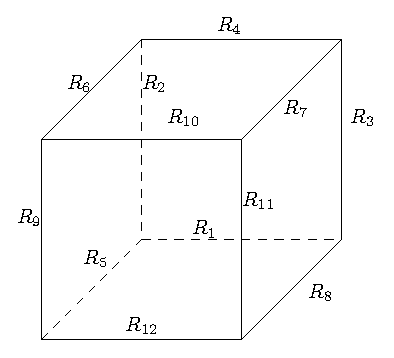
\includegraphics{./figures/wuerfel.eps}
\caption{Geometrie des Würfels mit Festlegung der Widerstände}
\label{fig:geometrie_wuerfel}
\end{figure}

\subsubsection{Oktaeder}
\begin{figure}[htbp!]
\centering
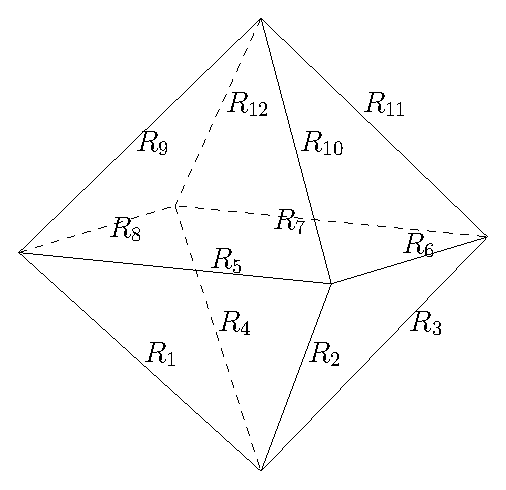
\includegraphics[width=0.3\textwidth]{./figures/oktaeder.eps}
\caption{Geometrie des Oktaeders mit Festlegung der Widerstände}
\label{fig:geometrie_oktaeder}
\end{figure}

\subsection{Physikalische Ergebnisse}

Wir setzen zur Bearbeitung der Aufgaben alle Widerstände auf $1$\si{\ohm}, wobei einer der Widerstände in Abschnitt \ref{sec:variation} varriert wird, und das Verhalten von $R_E$ bei dieser Änderung betrachtet wird.

\subsubsection{Analytische Lösung für gleiche Widerstände}
\label{auswertung}
\begin{wrapfigure}[12]{R}[1pt]{0.32\textwidth}
\centering
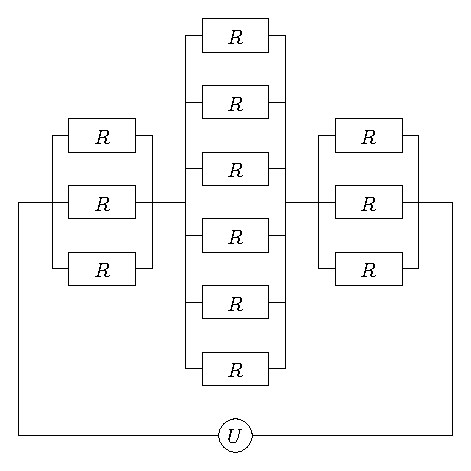
\includegraphics[width=0.3\textwidth]{./figures/ersatzschaltbild.eps}
\caption{Schaltbild für gleiche Widerstände $R$}
\label{fig:ersatzschaltbild}
\end{wrapfigure}
Für den Fall, dass alle verwendeten Widerstände gleich sind, lassen sich alle Ecken gleichen Potenzials verbinden und man erhält ein einfaches Ersatzschaltbild (Abb. \ref{fig:ersatzschaltbild}). Man nutzt nun aus, dass sich Widerstände in Parallelschaltungen reziprok und in Reihenschaltungen gewöhnlich addieren. Man erhält somit schnell:
\begin{align}
R_{ges}=\frac{R}{3}+\frac{R}{6}+\frac{R}{3}=\frac{5}{6}\,R
\end{align}

Für die Aufgabe gleicher Widerstände erhalten wir numerisch die gleiche Lösung, die sich bei analytischer Betrachtung ergibt. Zusammengefasst erhalten wir:
\begin{table}[htbp!]
\centering
\begin{tabular}{l|l}
Geometrie und Schaltung & Gesamtwiderstand $R_{ges}$\\\hline
\\
Würfel, Raumdiagonale & $5/6$
\end{tabular}
\end{table}

\subsubsection{Variation von $R_v$}
\label{sec:variation}
Wenn man einen beliebigen Widerstand $R_v$ ändert, hat dies je nach Lage des Widerstands einen anderen Einfluss auf den Gesamtwiderstand. Wir müssen also eine Fallunterscheidung für jede Schaltung einführen, die die Position des zu ändernden Widerstands im Netzwerk berücksichtigt. Dabei ist es aus Symmetriegründen möglich, dass zwei unterschiedliche Lagen von $R_v$ die gleiche Auswirkung auf den Gesamtwiderstand haben. In Tabelle \ref{tab:variation} ist für die verschiedenen Körper und Schaltungen dargestellt, welche Widerstände in unseren Schaltkreisen ausgetauscht werden können, ohne dass sich $R_E$ ändert.
\begin{table}[htbp!]
\centering
\begin{tabular}{llll}
\toprule
Geometrie & Spannung an & austauschbare Widerstände ohne Effekt auf $R_E$ & Position\footnotemark 
\\\midrule
 \multirow{2}{*}{Würfel} & \multirow{2}{*}{Raumdiagonale} & $R_1$, $R_3$, $R_5$, $R_7$, $R_9$, $R_{10}$ & 1\\
 & & $R_2$, $R_4$, $R_6$, $R_8$, $R_{11}$, $R_{12}$ & 2\\\midrule
 \multirow{4}{*}{Würfel}& \multirow{4}{*} {Flächendiagonale} & $R_1$, $R_{10}$ & 3\\
 & & $R_2$ $R_5$, $R_6$, $R_9$ & 4\\
 & & $R_3$, $R_7$, $R_8$, $R_{11}$ & 5\\
 & & $R_4$, $R_{12}$ & 6\\\midrule
 \multirow{5}{*}{Würfel} & \multirow{5}{*} {Kante} & $R_1$, $R_{10}$ & 7\\
 & & $R_2$ $R_3$, $R_6$, $R_7$ & 8\\
 & & $R_4$ & 9\\
 & & $R_5$, $R_8$, $R_9$, $R_{11}$ & 10\\
 & & $R_{12}$ & 11\\\midrule
 \multirow{2}{*}{Oktaeder} &\multirow{2}{*}{gegenüberliegende Spitzen} & $R_1$, $R_2$, $R_3$, $R_4$, $R_9$, $R_{10}$, $R_{11}$, $R_{12}$ & 12\\
 & & $R_5$, $R_6$, $R_7$, $R_8$ & 13\\\midrule
 \multirow{5}{*}{Oktaeder} & \multirow{5}{*} {Kante} & $R_1$, $R_3$, $R_7$, $R_8$ &14\\
 & & $R_2$, $R_{12}$ & 15\\
 & & $R_4$ & 16\\
 & & $R_5$, $R_6$, $R_9$, $R_{11}$ & 17\\
 & & $R_{10}$ & 18\\
\bottomrule
\end{tabular}

\caption{Widerstände in einer Zeile haben gleichen Auswirkungen auf $R_E$}
\label{tab:variation}
\end{table}
\footnotetext{zur Zuordnung der Plots}

\begin{thebibliography}{9}

\bibitem{lyness}
 Lyness, J. N.,
 \emph{Notes on the Adaptive Simpson Quadrature Routine},
Journal of the ACM
Volume 16 Issue 3, (1969) 
Seiten 483-495 

\end{thebibliography}
\newpage

\appendix
\section{Anhang: Grafische Darstellung der Variation von $R_1$}
\begin{figure}[htbp!]
\centering
% GNUPLOT: LaTeX picture with Postscript
\begingroup
  \makeatletter
  \providecommand\color[2][]{%
    \GenericError{(gnuplot) \space\space\space\@spaces}{%
      Package color not loaded in conjunction with
      terminal option `colourtext'%
    }{See the gnuplot documentation for explanation.%
    }{Either use 'blacktext' in gnuplot or load the package
      color.sty in LaTeX.}%
    \renewcommand\color[2][]{}%
  }%
  \providecommand\includegraphics[2][]{%
    \GenericError{(gnuplot) \space\space\space\@spaces}{%
      Package graphicx or graphics not loaded%
    }{See the gnuplot documentation for explanation.%
    }{The gnuplot epslatex terminal needs graphicx.sty or graphics.sty.}%
    \renewcommand\includegraphics[2][]{}%
  }%
  \providecommand\rotatebox[2]{#2}%
  \@ifundefined{ifGPcolor}{%
    \newif\ifGPcolor
    \GPcolortrue
  }{}%
  \@ifundefined{ifGPblacktext}{%
    \newif\ifGPblacktext
    \GPblacktextfalse
  }{}%
  % define a \g@addto@macro without @ in the name:
  \let\gplgaddtomacro\g@addto@macro
  % define empty templates for all commands taking text:
  \gdef\gplbacktext{}%
  \gdef\gplfronttext{}%
  \makeatother
  \ifGPblacktext
    % no textcolor at all
    \def\colorrgb#1{}%
    \def\colorgray#1{}%
  \else
    % gray or color?
    \ifGPcolor
      \def\colorrgb#1{\color[rgb]{#1}}%
      \def\colorgray#1{\color[gray]{#1}}%
      \expandafter\def\csname LTw\endcsname{\color{white}}%
      \expandafter\def\csname LTb\endcsname{\color{black}}%
      \expandafter\def\csname LTa\endcsname{\color{black}}%
      \expandafter\def\csname LT0\endcsname{\color[rgb]{1,0,0}}%
      \expandafter\def\csname LT1\endcsname{\color[rgb]{0,1,0}}%
      \expandafter\def\csname LT2\endcsname{\color[rgb]{0,0,1}}%
      \expandafter\def\csname LT3\endcsname{\color[rgb]{1,0,1}}%
      \expandafter\def\csname LT4\endcsname{\color[rgb]{0,1,1}}%
      \expandafter\def\csname LT5\endcsname{\color[rgb]{1,1,0}}%
      \expandafter\def\csname LT6\endcsname{\color[rgb]{0,0,0}}%
      \expandafter\def\csname LT7\endcsname{\color[rgb]{1,0.3,0}}%
      \expandafter\def\csname LT8\endcsname{\color[rgb]{0.5,0.5,0.5}}%
    \else
      % gray
      \def\colorrgb#1{\color{black}}%
      \def\colorgray#1{\color[gray]{#1}}%
      \expandafter\def\csname LTw\endcsname{\color{white}}%
      \expandafter\def\csname LTb\endcsname{\color{black}}%
      \expandafter\def\csname LTa\endcsname{\color{black}}%
      \expandafter\def\csname LT0\endcsname{\color{black}}%
      \expandafter\def\csname LT1\endcsname{\color{black}}%
      \expandafter\def\csname LT2\endcsname{\color{black}}%
      \expandafter\def\csname LT3\endcsname{\color{black}}%
      \expandafter\def\csname LT4\endcsname{\color{black}}%
      \expandafter\def\csname LT5\endcsname{\color{black}}%
      \expandafter\def\csname LT6\endcsname{\color{black}}%
      \expandafter\def\csname LT7\endcsname{\color{black}}%
      \expandafter\def\csname LT8\endcsname{\color{black}}%
    \fi
  \fi
  \setlength{\unitlength}{0.0500bp}%
  \begin{picture}(9360.00,4320.00)%
      \csname LTb\endcsname%
      \put(4680,4100){\makebox(0,0){\strut{}Verhalten von $R_E$ in Abhängigkeit von $R_v$}}%
    \gplgaddtomacro\gplbacktext{%
      \csname LTb\endcsname%
      \put(1078,704){\makebox(0,0)[r]{\strut{} 0.78}}%
      \csname LTb\endcsname%
      \put(1078,1233){\makebox(0,0)[r]{\strut{} 0.8}}%
      \csname LTb\endcsname%
      \put(1078,1762){\makebox(0,0)[r]{\strut{} 0.82}}%
      \csname LTb\endcsname%
      \put(1078,2292){\makebox(0,0)[r]{\strut{} 0.84}}%
      \csname LTb\endcsname%
      \put(1078,2821){\makebox(0,0)[r]{\strut{} 0.86}}%
      \csname LTb\endcsname%
      \put(1078,3350){\makebox(0,0)[r]{\strut{} 0.88}}%
      \csname LTb\endcsname%
      \put(1078,3879){\makebox(0,0)[r]{\strut{} 0.9}}%
      \csname LTb\endcsname%
      \put(1210,484){\makebox(0,0){\strut{} 0}}%
      \csname LTb\endcsname%
      \put(1978,484){\makebox(0,0){\strut{} 5}}%
      \csname LTb\endcsname%
      \put(2747,484){\makebox(0,0){\strut{} 10}}%
      \csname LTb\endcsname%
      \put(3515,484){\makebox(0,0){\strut{} 15}}%
      \csname LTb\endcsname%
      \put(4283,484){\makebox(0,0){\strut{} 20}}%
      \put(176,2291){\rotatebox{-270}{\makebox(0,0){\strut{}Ersatzwiderstand $R_E$ / \si{\ohm}}}}%
      \put(2746,154){\makebox(0,0){\strut{}Widerstandswert von $R_v$ / \si{\ohm}}}%
    }%
    \gplgaddtomacro\gplfronttext{%
      \csname LTb\endcsname%
      \put(3296,877){\makebox(0,0)[r]{\strut{}\footnotesize{Position $1$}}}%
    }%
    \gplgaddtomacro\gplbacktext{%
      \csname LTb\endcsname%
      \put(5538,704){\makebox(0,0)[r]{\strut{} 0.6}}%
      \csname LTb\endcsname%
      \put(5538,1022){\makebox(0,0)[r]{\strut{} 0.65}}%
      \csname LTb\endcsname%
      \put(5538,1339){\makebox(0,0)[r]{\strut{} 0.7}}%
      \csname LTb\endcsname%
      \put(5538,1657){\makebox(0,0)[r]{\strut{} 0.75}}%
      \csname LTb\endcsname%
      \put(5538,1974){\makebox(0,0)[r]{\strut{} 0.8}}%
      \csname LTb\endcsname%
      \put(5538,2292){\makebox(0,0)[r]{\strut{} 0.85}}%
      \csname LTb\endcsname%
      \put(5538,2609){\makebox(0,0)[r]{\strut{} 0.9}}%
      \csname LTb\endcsname%
      \put(5538,2927){\makebox(0,0)[r]{\strut{} 0.95}}%
      \csname LTb\endcsname%
      \put(5538,3244){\makebox(0,0)[r]{\strut{} 1}}%
      \csname LTb\endcsname%
      \put(5538,3562){\makebox(0,0)[r]{\strut{} 1.05}}%
      \csname LTb\endcsname%
      \put(5538,3879){\makebox(0,0)[r]{\strut{} 1.1}}%
      \csname LTb\endcsname%
      \put(5670,484){\makebox(0,0){\strut{} 0}}%
      \csname LTb\endcsname%
      \put(6493,484){\makebox(0,0){\strut{} 5}}%
      \csname LTb\endcsname%
      \put(7317,484){\makebox(0,0){\strut{} 10}}%
      \csname LTb\endcsname%
      \put(8140,484){\makebox(0,0){\strut{} 15}}%
      \csname LTb\endcsname%
      \put(8963,484){\makebox(0,0){\strut{} 20}}%
      \put(7316,154){\makebox(0,0){\strut{}Widerstandswert von $R_v$ / \si{\ohm}}}%
    }%
    \gplgaddtomacro\gplfronttext{%
      \csname LTb\endcsname%
      \put(7976,877){\makebox(0,0)[r]{\strut{}\footnotesize{Position $2$}}}%
    }%
    \gplbacktext
    \put(0,0){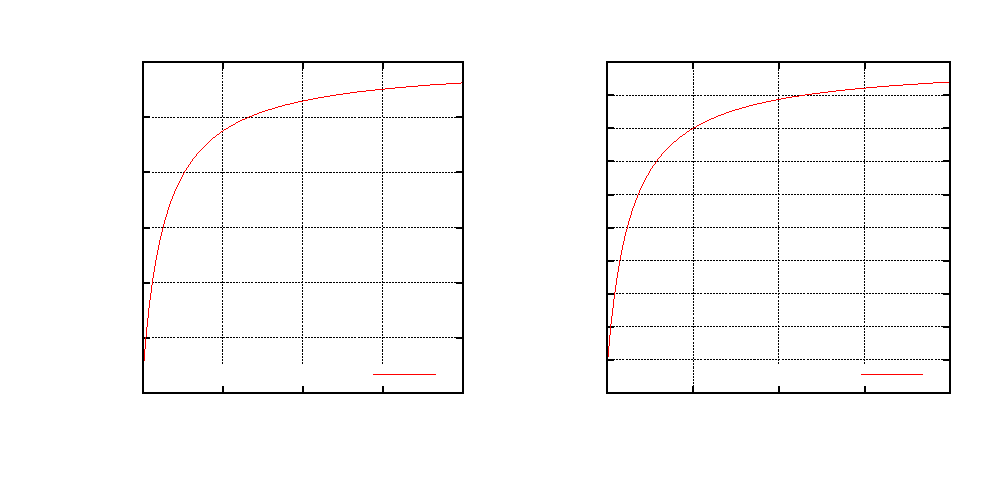
\includegraphics{./figures/wuerfel_diag}}%
    \gplfronttext
  \end{picture}%
\endgroup

\caption{Raumdiagonale Würfel}
\end{figure}
\begin{figure}[htbp!]
\centering
% GNUPLOT: LaTeX picture with Postscript
\begingroup
  \makeatletter
  \providecommand\color[2][]{%
    \GenericError{(gnuplot) \space\space\space\@spaces}{%
      Package color not loaded in conjunction with
      terminal option `colourtext'%
    }{See the gnuplot documentation for explanation.%
    }{Either use 'blacktext' in gnuplot or load the package
      color.sty in LaTeX.}%
    \renewcommand\color[2][]{}%
  }%
  \providecommand\includegraphics[2][]{%
    \GenericError{(gnuplot) \space\space\space\@spaces}{%
      Package graphicx or graphics not loaded%
    }{See the gnuplot documentation for explanation.%
    }{The gnuplot epslatex terminal needs graphicx.sty or graphics.sty.}%
    \renewcommand\includegraphics[2][]{}%
  }%
  \providecommand\rotatebox[2]{#2}%
  \@ifundefined{ifGPcolor}{%
    \newif\ifGPcolor
    \GPcolortrue
  }{}%
  \@ifundefined{ifGPblacktext}{%
    \newif\ifGPblacktext
    \GPblacktextfalse
  }{}%
  % define a \g@addto@macro without @ in the name:
  \let\gplgaddtomacro\g@addto@macro
  % define empty templates for all commands taking text:
  \gdef\gplbacktext{}%
  \gdef\gplfronttext{}%
  \makeatother
  \ifGPblacktext
    % no textcolor at all
    \def\colorrgb#1{}%
    \def\colorgray#1{}%
  \else
    % gray or color?
    \ifGPcolor
      \def\colorrgb#1{\color[rgb]{#1}}%
      \def\colorgray#1{\color[gray]{#1}}%
      \expandafter\def\csname LTw\endcsname{\color{white}}%
      \expandafter\def\csname LTb\endcsname{\color{black}}%
      \expandafter\def\csname LTa\endcsname{\color{black}}%
      \expandafter\def\csname LT0\endcsname{\color[rgb]{1,0,0}}%
      \expandafter\def\csname LT1\endcsname{\color[rgb]{0,1,0}}%
      \expandafter\def\csname LT2\endcsname{\color[rgb]{0,0,1}}%
      \expandafter\def\csname LT3\endcsname{\color[rgb]{1,0,1}}%
      \expandafter\def\csname LT4\endcsname{\color[rgb]{0,1,1}}%
      \expandafter\def\csname LT5\endcsname{\color[rgb]{1,1,0}}%
      \expandafter\def\csname LT6\endcsname{\color[rgb]{0,0,0}}%
      \expandafter\def\csname LT7\endcsname{\color[rgb]{1,0.3,0}}%
      \expandafter\def\csname LT8\endcsname{\color[rgb]{0.5,0.5,0.5}}%
    \else
      % gray
      \def\colorrgb#1{\color{black}}%
      \def\colorgray#1{\color[gray]{#1}}%
      \expandafter\def\csname LTw\endcsname{\color{white}}%
      \expandafter\def\csname LTb\endcsname{\color{black}}%
      \expandafter\def\csname LTa\endcsname{\color{black}}%
      \expandafter\def\csname LT0\endcsname{\color{black}}%
      \expandafter\def\csname LT1\endcsname{\color{black}}%
      \expandafter\def\csname LT2\endcsname{\color{black}}%
      \expandafter\def\csname LT3\endcsname{\color{black}}%
      \expandafter\def\csname LT4\endcsname{\color{black}}%
      \expandafter\def\csname LT5\endcsname{\color{black}}%
      \expandafter\def\csname LT6\endcsname{\color{black}}%
      \expandafter\def\csname LT7\endcsname{\color{black}}%
      \expandafter\def\csname LT8\endcsname{\color{black}}%
    \fi
  \fi
  \setlength{\unitlength}{0.0500bp}%
  \begin{picture}(9360.00,7920.00)%
      \csname LTb\endcsname%
      \put(4680,7700){\makebox(0,0){\strut{}Verhalten von $R_E$ in Abhängigkeit von $R_v$}}%
    \gplgaddtomacro\gplbacktext{%
      \csname LTb\endcsname%
      \put(1210,4290){\makebox(0,0)[r]{\strut{} 0.742}}%
      \csname LTb\endcsname%
      \put(1210,4689){\makebox(0,0)[r]{\strut{} 0.744}}%
      \csname LTb\endcsname%
      \put(1210,5087){\makebox(0,0)[r]{\strut{} 0.746}}%
      \csname LTb\endcsname%
      \put(1210,5486){\makebox(0,0)[r]{\strut{} 0.748}}%
      \csname LTb\endcsname%
      \put(1210,5885){\makebox(0,0)[r]{\strut{} 0.75}}%
      \csname LTb\endcsname%
      \put(1210,6283){\makebox(0,0)[r]{\strut{} 0.752}}%
      \csname LTb\endcsname%
      \put(1210,6682){\makebox(0,0)[r]{\strut{} 0.754}}%
      \csname LTb\endcsname%
      \put(1210,7080){\makebox(0,0)[r]{\strut{} 0.756}}%
      \csname LTb\endcsname%
      \put(1210,7479){\makebox(0,0)[r]{\strut{} 0.758}}%
      \csname LTb\endcsname%
      \put(1342,4070){\makebox(0,0){\strut{} 0}}%
      \csname LTb\endcsname%
      \put(2077,4070){\makebox(0,0){\strut{} 5}}%
      \csname LTb\endcsname%
      \put(2813,4070){\makebox(0,0){\strut{} 10}}%
      \csname LTb\endcsname%
      \put(3548,4070){\makebox(0,0){\strut{} 15}}%
      \csname LTb\endcsname%
      \put(4283,4070){\makebox(0,0){\strut{} 20}}%
      \put(176,5884){\rotatebox{-270}{\makebox(0,0){\strut{}Ersatzwiderstand $R_E$ / \si{\ohm}}}}%
    }%
    \gplgaddtomacro\gplfronttext{%
      \csname LTb\endcsname%
      \put(3296,4463){\makebox(0,0)[r]{\strut{}\footnotesize{Position $3$}}}%
    }%
    \gplgaddtomacro\gplbacktext{%
      \csname LTb\endcsname%
      \put(5406,4290){\makebox(0,0)[r]{\strut{} 0.5}}%
      \csname LTb\endcsname%
      \put(5406,4822){\makebox(0,0)[r]{\strut{} 0.6}}%
      \csname LTb\endcsname%
      \put(5406,5353){\makebox(0,0)[r]{\strut{} 0.7}}%
      \csname LTb\endcsname%
      \put(5406,5884){\makebox(0,0)[r]{\strut{} 0.8}}%
      \csname LTb\endcsname%
      \put(5406,6416){\makebox(0,0)[r]{\strut{} 0.9}}%
      \csname LTb\endcsname%
      \put(5406,6947){\makebox(0,0)[r]{\strut{} 1}}%
      \csname LTb\endcsname%
      \put(5406,7479){\makebox(0,0)[r]{\strut{} 1.1}}%
      \csname LTb\endcsname%
      \put(5538,4070){\makebox(0,0){\strut{} 0}}%
      \csname LTb\endcsname%
      \put(6394,4070){\makebox(0,0){\strut{} 5}}%
      \csname LTb\endcsname%
      \put(7251,4070){\makebox(0,0){\strut{} 10}}%
      \csname LTb\endcsname%
      \put(8107,4070){\makebox(0,0){\strut{} 15}}%
      \csname LTb\endcsname%
      \put(8963,4070){\makebox(0,0){\strut{} 20}}%
    }%
    \gplgaddtomacro\gplfronttext{%
      \csname LTb\endcsname%
      \put(7976,4463){\makebox(0,0)[r]{\strut{}\footnotesize{Position $4$}}}%
    }%
    \gplgaddtomacro\gplbacktext{%
      \csname LTb\endcsname%
      \put(1078,704){\makebox(0,0)[r]{\strut{} 0.72}}%
      \csname LTb\endcsname%
      \put(1078,1122){\makebox(0,0)[r]{\strut{} 0.73}}%
      \csname LTb\endcsname%
      \put(1078,1540){\makebox(0,0)[r]{\strut{} 0.74}}%
      \csname LTb\endcsname%
      \put(1078,1958){\makebox(0,0)[r]{\strut{} 0.75}}%
      \csname LTb\endcsname%
      \put(1078,2376){\makebox(0,0)[r]{\strut{} 0.76}}%
      \csname LTb\endcsname%
      \put(1078,2794){\makebox(0,0)[r]{\strut{} 0.77}}%
      \csname LTb\endcsname%
      \put(1078,3212){\makebox(0,0)[r]{\strut{} 0.78}}%
      \csname LTb\endcsname%
      \put(1078,3630){\makebox(0,0)[r]{\strut{} 0.79}}%
      \csname LTb\endcsname%
      \put(1210,484){\makebox(0,0){\strut{} 0}}%
      \csname LTb\endcsname%
      \put(1978,484){\makebox(0,0){\strut{} 5}}%
      \csname LTb\endcsname%
      \put(2747,484){\makebox(0,0){\strut{} 10}}%
      \csname LTb\endcsname%
      \put(3515,484){\makebox(0,0){\strut{} 15}}%
      \csname LTb\endcsname%
      \put(4283,484){\makebox(0,0){\strut{} 20}}%
      \put(176,2167){\rotatebox{-270}{\makebox(0,0){\strut{}Ersatzwiderstand $R_E$ / \si{\ohm}}}}%
      \put(2746,154){\makebox(0,0){\strut{}Widerstandswert von $R_v$ / \si{\ohm}}}%
    }%
    \gplgaddtomacro\gplfronttext{%
      \csname LTb\endcsname%
      \put(3296,877){\makebox(0,0)[r]{\strut{}\footnotesize{Position $5$}}}%
    }%
    \gplgaddtomacro\gplbacktext{%
      \csname LTb\endcsname%
      \put(5538,704){\makebox(0,0)[r]{\strut{} 0.6}}%
      \csname LTb\endcsname%
      \put(5538,1192){\makebox(0,0)[r]{\strut{} 0.65}}%
      \csname LTb\endcsname%
      \put(5538,1679){\makebox(0,0)[r]{\strut{} 0.7}}%
      \csname LTb\endcsname%
      \put(5538,2167){\makebox(0,0)[r]{\strut{} 0.75}}%
      \csname LTb\endcsname%
      \put(5538,2655){\makebox(0,0)[r]{\strut{} 0.8}}%
      \csname LTb\endcsname%
      \put(5538,3142){\makebox(0,0)[r]{\strut{} 0.85}}%
      \csname LTb\endcsname%
      \put(5538,3630){\makebox(0,0)[r]{\strut{} 0.9}}%
      \csname LTb\endcsname%
      \put(5670,484){\makebox(0,0){\strut{} 0}}%
      \csname LTb\endcsname%
      \put(6493,484){\makebox(0,0){\strut{} 5}}%
      \csname LTb\endcsname%
      \put(7317,484){\makebox(0,0){\strut{} 10}}%
      \csname LTb\endcsname%
      \put(8140,484){\makebox(0,0){\strut{} 15}}%
      \csname LTb\endcsname%
      \put(8963,484){\makebox(0,0){\strut{} 20}}%
      \put(7316,154){\makebox(0,0){\strut{}Widerstandswert von $R_v$ / \si{\ohm}}}%
    }%
    \gplgaddtomacro\gplfronttext{%
      \csname LTb\endcsname%
      \put(7976,877){\makebox(0,0)[r]{\strut{}\footnotesize{Position $6$}}}%
    }%
    \gplbacktext
    \put(0,0){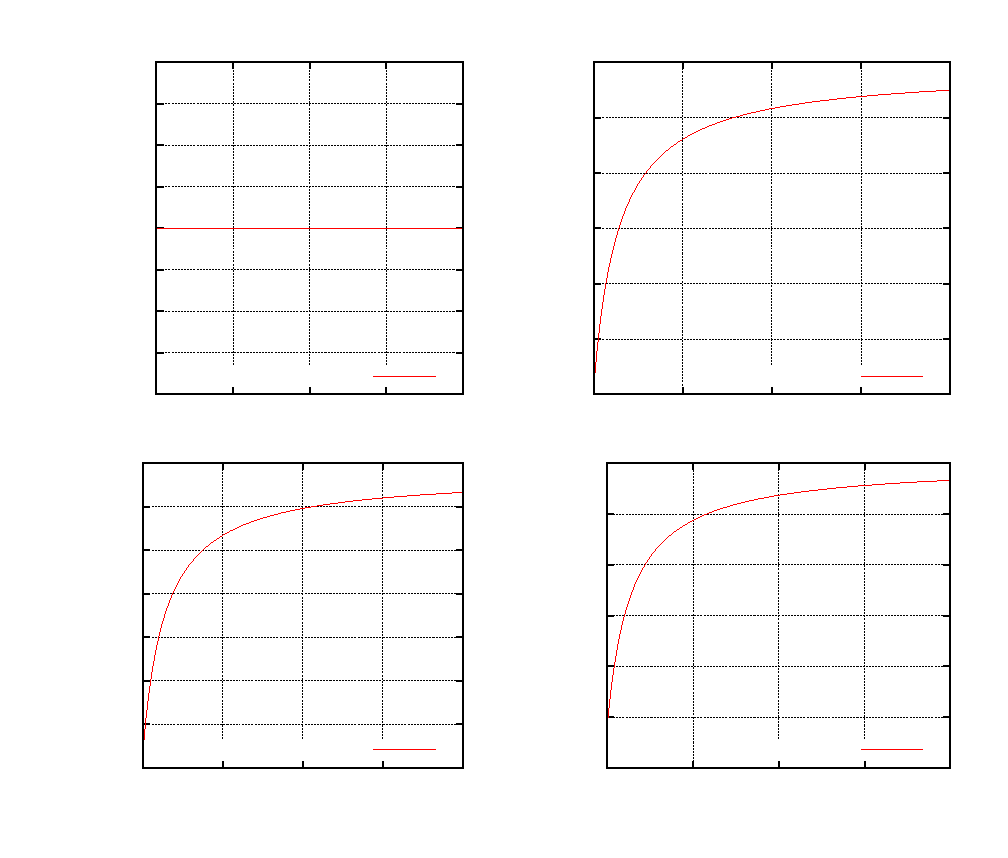
\includegraphics{./figures/wuerfel_face}}%
    \gplfronttext
  \end{picture}%
\endgroup

\caption{Flächendiagonale Würfel}
\end{figure}
\begin{figure}[htbp!]
\centering
% GNUPLOT: LaTeX picture with Postscript
\begingroup
  \makeatletter
  \providecommand\color[2][]{%
    \GenericError{(gnuplot) \space\space\space\@spaces}{%
      Package color not loaded in conjunction with
      terminal option `colourtext'%
    }{See the gnuplot documentation for explanation.%
    }{Either use 'blacktext' in gnuplot or load the package
      color.sty in LaTeX.}%
    \renewcommand\color[2][]{}%
  }%
  \providecommand\includegraphics[2][]{%
    \GenericError{(gnuplot) \space\space\space\@spaces}{%
      Package graphicx or graphics not loaded%
    }{See the gnuplot documentation for explanation.%
    }{The gnuplot epslatex terminal needs graphicx.sty or graphics.sty.}%
    \renewcommand\includegraphics[2][]{}%
  }%
  \providecommand\rotatebox[2]{#2}%
  \@ifundefined{ifGPcolor}{%
    \newif\ifGPcolor
    \GPcolortrue
  }{}%
  \@ifundefined{ifGPblacktext}{%
    \newif\ifGPblacktext
    \GPblacktextfalse
  }{}%
  % define a \g@addto@macro without @ in the name:
  \let\gplgaddtomacro\g@addto@macro
  % define empty templates for all commands taking text:
  \gdef\gplbacktext{}%
  \gdef\gplfronttext{}%
  \makeatother
  \ifGPblacktext
    % no textcolor at all
    \def\colorrgb#1{}%
    \def\colorgray#1{}%
  \else
    % gray or color?
    \ifGPcolor
      \def\colorrgb#1{\color[rgb]{#1}}%
      \def\colorgray#1{\color[gray]{#1}}%
      \expandafter\def\csname LTw\endcsname{\color{white}}%
      \expandafter\def\csname LTb\endcsname{\color{black}}%
      \expandafter\def\csname LTa\endcsname{\color{black}}%
      \expandafter\def\csname LT0\endcsname{\color[rgb]{1,0,0}}%
      \expandafter\def\csname LT1\endcsname{\color[rgb]{0,1,0}}%
      \expandafter\def\csname LT2\endcsname{\color[rgb]{0,0,1}}%
      \expandafter\def\csname LT3\endcsname{\color[rgb]{1,0,1}}%
      \expandafter\def\csname LT4\endcsname{\color[rgb]{0,1,1}}%
      \expandafter\def\csname LT5\endcsname{\color[rgb]{1,1,0}}%
      \expandafter\def\csname LT6\endcsname{\color[rgb]{0,0,0}}%
      \expandafter\def\csname LT7\endcsname{\color[rgb]{1,0.3,0}}%
      \expandafter\def\csname LT8\endcsname{\color[rgb]{0.5,0.5,0.5}}%
    \else
      % gray
      \def\colorrgb#1{\color{black}}%
      \def\colorgray#1{\color[gray]{#1}}%
      \expandafter\def\csname LTw\endcsname{\color{white}}%
      \expandafter\def\csname LTb\endcsname{\color{black}}%
      \expandafter\def\csname LTa\endcsname{\color{black}}%
      \expandafter\def\csname LT0\endcsname{\color{black}}%
      \expandafter\def\csname LT1\endcsname{\color{black}}%
      \expandafter\def\csname LT2\endcsname{\color{black}}%
      \expandafter\def\csname LT3\endcsname{\color{black}}%
      \expandafter\def\csname LT4\endcsname{\color{black}}%
      \expandafter\def\csname LT5\endcsname{\color{black}}%
      \expandafter\def\csname LT6\endcsname{\color{black}}%
      \expandafter\def\csname LT7\endcsname{\color{black}}%
      \expandafter\def\csname LT8\endcsname{\color{black}}%
    \fi
  \fi
  \setlength{\unitlength}{0.0500bp}%
  \begin{picture}(9360.00,11520.00)%
      \csname LTb\endcsname%
      \put(4680,11300){\makebox(0,0){\strut{}Verhalten von $R_E$ in Abhängigkeit von $R_1$}}%
    \gplgaddtomacro\gplbacktext{%
      \csname LTb\endcsname%
      \put(1078,7973){\makebox(0,0)[r]{\strut{} 0.52}}%
      \csname LTb\endcsname%
      \put(1078,8417){\makebox(0,0)[r]{\strut{} 0.54}}%
      \csname LTb\endcsname%
      \put(1078,8860){\makebox(0,0)[r]{\strut{} 0.56}}%
      \csname LTb\endcsname%
      \put(1078,9304){\makebox(0,0)[r]{\strut{} 0.58}}%
      \csname LTb\endcsname%
      \put(1078,9748){\makebox(0,0)[r]{\strut{} 0.6}}%
      \csname LTb\endcsname%
      \put(1078,10192){\makebox(0,0)[r]{\strut{} 0.62}}%
      \csname LTb\endcsname%
      \put(1078,10635){\makebox(0,0)[r]{\strut{} 0.64}}%
      \csname LTb\endcsname%
      \put(1078,11079){\makebox(0,0)[r]{\strut{} 0.66}}%
      \csname LTb\endcsname%
      \put(1210,7753){\makebox(0,0){\strut{} 0}}%
      \csname LTb\endcsname%
      \put(1978,7753){\makebox(0,0){\strut{} 5}}%
      \csname LTb\endcsname%
      \put(2747,7753){\makebox(0,0){\strut{} 10}}%
      \csname LTb\endcsname%
      \put(3515,7753){\makebox(0,0){\strut{} 15}}%
      \csname LTb\endcsname%
      \put(4283,7753){\makebox(0,0){\strut{} 20}}%
      \put(176,9526){\rotatebox{-270}{\makebox(0,0){\strut{}Ersatzwiderstand $R_E$ / \si{\ohm}}}}%
    }%
    \gplgaddtomacro\gplfronttext{%
      \csname LTb\endcsname%
      \put(3296,8146){\makebox(0,0)[r]{\strut{}\footnotesize{Position $7$}}}%
    }%
    \gplgaddtomacro\gplbacktext{%
      \csname LTb\endcsname%
      \put(5670,7973){\makebox(0,0)[r]{\strut{} 0.58}}%
      \csname LTb\endcsname%
      \put(5670,8361){\makebox(0,0)[r]{\strut{} 0.581}}%
      \csname LTb\endcsname%
      \put(5670,8750){\makebox(0,0)[r]{\strut{} 0.582}}%
      \csname LTb\endcsname%
      \put(5670,9138){\makebox(0,0)[r]{\strut{} 0.583}}%
      \csname LTb\endcsname%
      \put(5670,9526){\makebox(0,0)[r]{\strut{} 0.584}}%
      \csname LTb\endcsname%
      \put(5670,9914){\makebox(0,0)[r]{\strut{} 0.585}}%
      \csname LTb\endcsname%
      \put(5670,10303){\makebox(0,0)[r]{\strut{} 0.586}}%
      \csname LTb\endcsname%
      \put(5670,10691){\makebox(0,0)[r]{\strut{} 0.587}}%
      \csname LTb\endcsname%
      \put(5670,11079){\makebox(0,0)[r]{\strut{} 0.588}}%
      \csname LTb\endcsname%
      \put(5802,7753){\makebox(0,0){\strut{} 0}}%
      \csname LTb\endcsname%
      \put(6592,7753){\makebox(0,0){\strut{} 5}}%
      \csname LTb\endcsname%
      \put(7383,7753){\makebox(0,0){\strut{} 10}}%
      \csname LTb\endcsname%
      \put(8173,7753){\makebox(0,0){\strut{} 15}}%
      \csname LTb\endcsname%
      \put(8963,7753){\makebox(0,0){\strut{} 20}}%
    }%
    \gplgaddtomacro\gplfronttext{%
      \csname LTb\endcsname%
      \put(7976,8146){\makebox(0,0)[r]{\strut{}\footnotesize{Position $8$}}}%
    }%
    \gplgaddtomacro\gplbacktext{%
      \csname LTb\endcsname%
      \put(1210,4206){\makebox(0,0)[r]{\strut{} 0.57}}%
      \csname LTb\endcsname%
      \put(1210,4724){\makebox(0,0)[r]{\strut{} 0.575}}%
      \csname LTb\endcsname%
      \put(1210,5242){\makebox(0,0)[r]{\strut{} 0.58}}%
      \csname LTb\endcsname%
      \put(1210,5760){\makebox(0,0)[r]{\strut{} 0.585}}%
      \csname LTb\endcsname%
      \put(1210,6277){\makebox(0,0)[r]{\strut{} 0.59}}%
      \csname LTb\endcsname%
      \put(1210,6795){\makebox(0,0)[r]{\strut{} 0.595}}%
      \csname LTb\endcsname%
      \put(1210,7313){\makebox(0,0)[r]{\strut{} 0.6}}%
      \csname LTb\endcsname%
      \put(1342,3986){\makebox(0,0){\strut{} 0}}%
      \csname LTb\endcsname%
      \put(2077,3986){\makebox(0,0){\strut{} 5}}%
      \csname LTb\endcsname%
      \put(2813,3986){\makebox(0,0){\strut{} 10}}%
      \csname LTb\endcsname%
      \put(3548,3986){\makebox(0,0){\strut{} 15}}%
      \csname LTb\endcsname%
      \put(4283,3986){\makebox(0,0){\strut{} 20}}%
      \put(176,5759){\rotatebox{-270}{\makebox(0,0){\strut{}Ersatzwiderstand $R_E$ / \si{\ohm}}}}%
    }%
    \gplgaddtomacro\gplfronttext{%
      \csname LTb\endcsname%
      \put(3296,4379){\makebox(0,0)[r]{\strut{}\footnotesize{Position $9$}}}%
    }%
    \gplgaddtomacro\gplbacktext{%
      \csname LTb\endcsname%
      \put(5538,4470){\makebox(0,0)[r]{\strut{} 0.5}}%
      \csname LTb\endcsname%
      \put(5538,4786){\makebox(0,0)[r]{\strut{} 0.52}}%
      \csname LTb\endcsname%
      \put(5538,5102){\makebox(0,0)[r]{\strut{} 0.54}}%
      \csname LTb\endcsname%
      \put(5538,5418){\makebox(0,0)[r]{\strut{} 0.56}}%
      \csname LTb\endcsname%
      \put(5538,5734){\makebox(0,0)[r]{\strut{} 0.58}}%
      \csname LTb\endcsname%
      \put(5538,6049){\makebox(0,0)[r]{\strut{} 0.6}}%
      \csname LTb\endcsname%
      \put(5538,6365){\makebox(0,0)[r]{\strut{} 0.62}}%
      \csname LTb\endcsname%
      \put(5538,6681){\makebox(0,0)[r]{\strut{} 0.64}}%
      \csname LTb\endcsname%
      \put(5538,6997){\makebox(0,0)[r]{\strut{} 0.66}}%
      \csname LTb\endcsname%
      \put(5538,7313){\makebox(0,0)[r]{\strut{} 0.68}}%
      \csname LTb\endcsname%
      \put(5670,4250){\makebox(0,0){\strut{} 0}}%
      \csname LTb\endcsname%
      \put(6493,4250){\makebox(0,0){\strut{} 5}}%
      \csname LTb\endcsname%
      \put(7317,4250){\makebox(0,0){\strut{} 10}}%
      \csname LTb\endcsname%
      \put(8140,4250){\makebox(0,0){\strut{} 15}}%
      \csname LTb\endcsname%
      \put(8963,4250){\makebox(0,0){\strut{} 20}}%
      \put(7316,3920){\makebox(0,0){\strut{}Widerstandswert von $R_1$ / \si{\ohm}}}%
    }%
    \gplgaddtomacro\gplfronttext{%
      \csname LTb\endcsname%
      \put(7976,4643){\makebox(0,0)[r]{\strut{}\footnotesize{Position $10$}}}%
    }%
    \gplgaddtomacro\gplbacktext{%
      \csname LTb\endcsname%
      \put(946,704){\makebox(0,0)[r]{\strut{} 0}}%
      \csname LTb\endcsname%
      \put(946,1110){\makebox(0,0)[r]{\strut{} 0.2}}%
      \csname LTb\endcsname%
      \put(946,1516){\makebox(0,0)[r]{\strut{} 0.4}}%
      \csname LTb\endcsname%
      \put(946,1922){\makebox(0,0)[r]{\strut{} 0.6}}%
      \csname LTb\endcsname%
      \put(946,2328){\makebox(0,0)[r]{\strut{} 0.8}}%
      \csname LTb\endcsname%
      \put(946,2734){\makebox(0,0)[r]{\strut{} 1}}%
      \csname LTb\endcsname%
      \put(946,3140){\makebox(0,0)[r]{\strut{} 1.2}}%
      \csname LTb\endcsname%
      \put(946,3546){\makebox(0,0)[r]{\strut{} 1.4}}%
      \csname LTb\endcsname%
      \put(1078,484){\makebox(0,0){\strut{} 0}}%
      \csname LTb\endcsname%
      \put(1879,484){\makebox(0,0){\strut{} 5}}%
      \csname LTb\endcsname%
      \put(2681,484){\makebox(0,0){\strut{} 10}}%
      \csname LTb\endcsname%
      \put(3482,484){\makebox(0,0){\strut{} 15}}%
      \csname LTb\endcsname%
      \put(4283,484){\makebox(0,0){\strut{} 20}}%
      \put(176,2125){\rotatebox{-270}{\makebox(0,0){\strut{}Ersatzwiderstand $R_E$ / \si{\ohm}}}}%
      \put(2680,154){\makebox(0,0){\strut{}Widerstandswert von $R_1$ / \si{\ohm}}}%
    }%
    \gplgaddtomacro\gplfronttext{%
      \csname LTb\endcsname%
      \put(3296,877){\makebox(0,0)[r]{\strut{}\footnotesize{Position $11$}}}%
    }%
    \gplbacktext
    \put(0,0){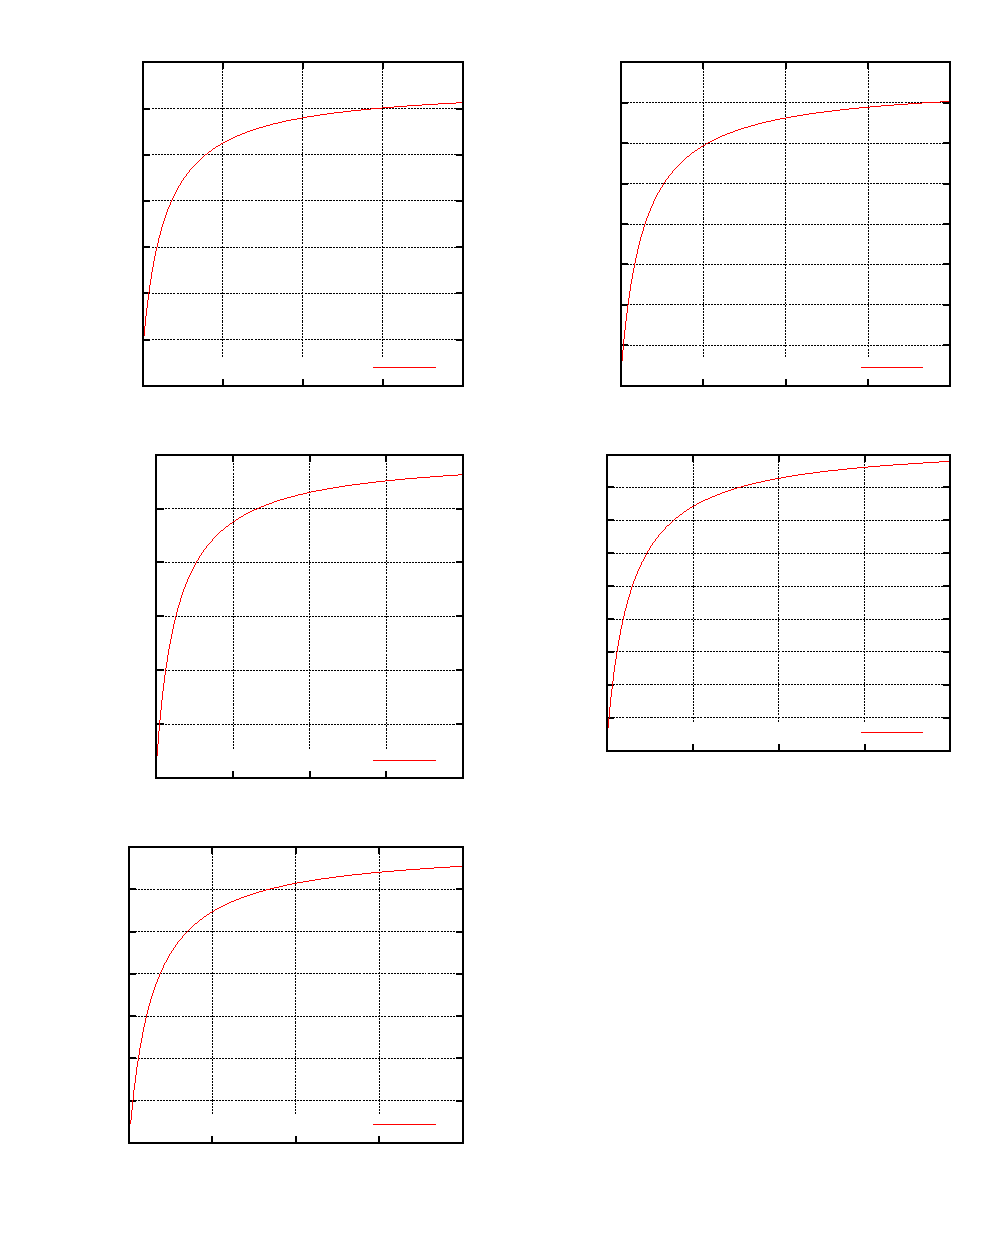
\includegraphics{./figures/wuerfel_edge}}%
    \gplfronttext
  \end{picture}%
\endgroup

\caption{Kante Würfel}
\end{figure}
\begin{figure}[htbp!]
\centering
% GNUPLOT: LaTeX picture with Postscript
\begingroup
  \makeatletter
  \providecommand\color[2][]{%
    \GenericError{(gnuplot) \space\space\space\@spaces}{%
      Package color not loaded in conjunction with
      terminal option `colourtext'%
    }{See the gnuplot documentation for explanation.%
    }{Either use 'blacktext' in gnuplot or load the package
      color.sty in LaTeX.}%
    \renewcommand\color[2][]{}%
  }%
  \providecommand\includegraphics[2][]{%
    \GenericError{(gnuplot) \space\space\space\@spaces}{%
      Package graphicx or graphics not loaded%
    }{See the gnuplot documentation for explanation.%
    }{The gnuplot epslatex terminal needs graphicx.sty or graphics.sty.}%
    \renewcommand\includegraphics[2][]{}%
  }%
  \providecommand\rotatebox[2]{#2}%
  \@ifundefined{ifGPcolor}{%
    \newif\ifGPcolor
    \GPcolortrue
  }{}%
  \@ifundefined{ifGPblacktext}{%
    \newif\ifGPblacktext
    \GPblacktextfalse
  }{}%
  % define a \g@addto@macro without @ in the name:
  \let\gplgaddtomacro\g@addto@macro
  % define empty templates for all commands taking text:
  \gdef\gplbacktext{}%
  \gdef\gplfronttext{}%
  \makeatother
  \ifGPblacktext
    % no textcolor at all
    \def\colorrgb#1{}%
    \def\colorgray#1{}%
  \else
    % gray or color?
    \ifGPcolor
      \def\colorrgb#1{\color[rgb]{#1}}%
      \def\colorgray#1{\color[gray]{#1}}%
      \expandafter\def\csname LTw\endcsname{\color{white}}%
      \expandafter\def\csname LTb\endcsname{\color{black}}%
      \expandafter\def\csname LTa\endcsname{\color{black}}%
      \expandafter\def\csname LT0\endcsname{\color[rgb]{1,0,0}}%
      \expandafter\def\csname LT1\endcsname{\color[rgb]{0,1,0}}%
      \expandafter\def\csname LT2\endcsname{\color[rgb]{0,0,1}}%
      \expandafter\def\csname LT3\endcsname{\color[rgb]{1,0,1}}%
      \expandafter\def\csname LT4\endcsname{\color[rgb]{0,1,1}}%
      \expandafter\def\csname LT5\endcsname{\color[rgb]{1,1,0}}%
      \expandafter\def\csname LT6\endcsname{\color[rgb]{0,0,0}}%
      \expandafter\def\csname LT7\endcsname{\color[rgb]{1,0.3,0}}%
      \expandafter\def\csname LT8\endcsname{\color[rgb]{0.5,0.5,0.5}}%
    \else
      % gray
      \def\colorrgb#1{\color{black}}%
      \def\colorgray#1{\color[gray]{#1}}%
      \expandafter\def\csname LTw\endcsname{\color{white}}%
      \expandafter\def\csname LTb\endcsname{\color{black}}%
      \expandafter\def\csname LTa\endcsname{\color{black}}%
      \expandafter\def\csname LT0\endcsname{\color{black}}%
      \expandafter\def\csname LT1\endcsname{\color{black}}%
      \expandafter\def\csname LT2\endcsname{\color{black}}%
      \expandafter\def\csname LT3\endcsname{\color{black}}%
      \expandafter\def\csname LT4\endcsname{\color{black}}%
      \expandafter\def\csname LT5\endcsname{\color{black}}%
      \expandafter\def\csname LT6\endcsname{\color{black}}%
      \expandafter\def\csname LT7\endcsname{\color{black}}%
      \expandafter\def\csname LT8\endcsname{\color{black}}%
    \fi
  \fi
  \setlength{\unitlength}{0.0500bp}%
  \begin{picture}(9360.00,4320.00)%
      \csname LTb\endcsname%
      \put(4680,4100){\makebox(0,0){\strut{}Verhalten von $R_E$ in Abhängigkeit von $R_1$}}%
    \gplgaddtomacro\gplbacktext{%
      \csname LTb\endcsname%
      \put(1078,704){\makebox(0,0)[r]{\strut{} 0.3}}%
      \csname LTb\endcsname%
      \put(1078,1233){\makebox(0,0)[r]{\strut{} 0.35}}%
      \csname LTb\endcsname%
      \put(1078,1762){\makebox(0,0)[r]{\strut{} 0.4}}%
      \csname LTb\endcsname%
      \put(1078,2291){\makebox(0,0)[r]{\strut{} 0.45}}%
      \csname LTb\endcsname%
      \put(1078,2821){\makebox(0,0)[r]{\strut{} 0.5}}%
      \csname LTb\endcsname%
      \put(1078,3350){\makebox(0,0)[r]{\strut{} 0.55}}%
      \csname LTb\endcsname%
      \put(1078,3879){\makebox(0,0)[r]{\strut{} 0.6}}%
      \csname LTb\endcsname%
      \put(1210,484){\makebox(0,0){\strut{} 0}}%
      \csname LTb\endcsname%
      \put(1978,484){\makebox(0,0){\strut{} 5}}%
      \csname LTb\endcsname%
      \put(2747,484){\makebox(0,0){\strut{} 10}}%
      \csname LTb\endcsname%
      \put(3515,484){\makebox(0,0){\strut{} 15}}%
      \csname LTb\endcsname%
      \put(4283,484){\makebox(0,0){\strut{} 20}}%
      \put(176,2291){\rotatebox{-270}{\makebox(0,0){\strut{}Ersatzwiderstand $R_E$ / \si{\ohm}}}}%
      \put(2746,154){\makebox(0,0){\strut{}Widerstandswert von $R_1$ / \si{\ohm}}}%
    }%
    \gplgaddtomacro\gplfronttext{%
      \csname LTb\endcsname%
      \put(3296,877){\makebox(0,0)[r]{\strut{}\footnotesize{Position $12$}}}%
    }%
    \gplgaddtomacro\gplbacktext{%
      \csname LTb\endcsname%
      \put(5670,704){\makebox(0,0)[r]{\strut{} 0.494}}%
      \csname LTb\endcsname%
      \put(5670,1233){\makebox(0,0)[r]{\strut{} 0.496}}%
      \csname LTb\endcsname%
      \put(5670,1762){\makebox(0,0)[r]{\strut{} 0.498}}%
      \csname LTb\endcsname%
      \put(5670,2292){\makebox(0,0)[r]{\strut{} 0.5}}%
      \csname LTb\endcsname%
      \put(5670,2821){\makebox(0,0)[r]{\strut{} 0.502}}%
      \csname LTb\endcsname%
      \put(5670,3350){\makebox(0,0)[r]{\strut{} 0.504}}%
      \csname LTb\endcsname%
      \put(5670,3879){\makebox(0,0)[r]{\strut{} 0.506}}%
      \csname LTb\endcsname%
      \put(5802,484){\makebox(0,0){\strut{} 0}}%
      \csname LTb\endcsname%
      \put(6592,484){\makebox(0,0){\strut{} 5}}%
      \csname LTb\endcsname%
      \put(7383,484){\makebox(0,0){\strut{} 10}}%
      \csname LTb\endcsname%
      \put(8173,484){\makebox(0,0){\strut{} 15}}%
      \csname LTb\endcsname%
      \put(8963,484){\makebox(0,0){\strut{} 20}}%
      \put(7382,154){\makebox(0,0){\strut{}Widerstandswert von $R_1$ / \si{\ohm}}}%
    }%
    \gplgaddtomacro\gplfronttext{%
      \csname LTb\endcsname%
      \put(7976,877){\makebox(0,0)[r]{\strut{}\footnotesize{Position $13$}}}%
    }%
    \gplbacktext
    \put(0,0){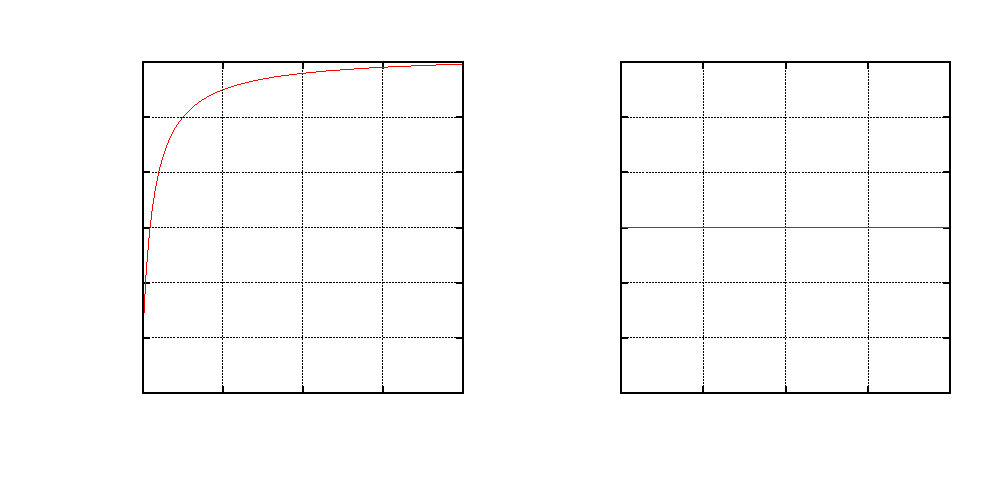
\includegraphics{./figures/oct_diag}}%
    \gplfronttext
  \end{picture}%
\endgroup

\caption{Diagonale Oktaeder}
\end{figure}
\begin{figure}[htbp!]
\centering
% GNUPLOT: LaTeX picture with Postscript
\begingroup
  \makeatletter
  \providecommand\color[2][]{%
    \GenericError{(gnuplot) \space\space\space\@spaces}{%
      Package color not loaded in conjunction with
      terminal option `colourtext'%
    }{See the gnuplot documentation for explanation.%
    }{Either use 'blacktext' in gnuplot or load the package
      color.sty in LaTeX.}%
    \renewcommand\color[2][]{}%
  }%
  \providecommand\includegraphics[2][]{%
    \GenericError{(gnuplot) \space\space\space\@spaces}{%
      Package graphicx or graphics not loaded%
    }{See the gnuplot documentation for explanation.%
    }{The gnuplot epslatex terminal needs graphicx.sty or graphics.sty.}%
    \renewcommand\includegraphics[2][]{}%
  }%
  \providecommand\rotatebox[2]{#2}%
  \@ifundefined{ifGPcolor}{%
    \newif\ifGPcolor
    \GPcolortrue
  }{}%
  \@ifundefined{ifGPblacktext}{%
    \newif\ifGPblacktext
    \GPblacktextfalse
  }{}%
  % define a \g@addto@macro without @ in the name:
  \let\gplgaddtomacro\g@addto@macro
  % define empty templates for all commands taking text:
  \gdef\gplbacktext{}%
  \gdef\gplfronttext{}%
  \makeatother
  \ifGPblacktext
    % no textcolor at all
    \def\colorrgb#1{}%
    \def\colorgray#1{}%
  \else
    % gray or color?
    \ifGPcolor
      \def\colorrgb#1{\color[rgb]{#1}}%
      \def\colorgray#1{\color[gray]{#1}}%
      \expandafter\def\csname LTw\endcsname{\color{white}}%
      \expandafter\def\csname LTb\endcsname{\color{black}}%
      \expandafter\def\csname LTa\endcsname{\color{black}}%
      \expandafter\def\csname LT0\endcsname{\color[rgb]{1,0,0}}%
      \expandafter\def\csname LT1\endcsname{\color[rgb]{0,1,0}}%
      \expandafter\def\csname LT2\endcsname{\color[rgb]{0,0,1}}%
      \expandafter\def\csname LT3\endcsname{\color[rgb]{1,0,1}}%
      \expandafter\def\csname LT4\endcsname{\color[rgb]{0,1,1}}%
      \expandafter\def\csname LT5\endcsname{\color[rgb]{1,1,0}}%
      \expandafter\def\csname LT6\endcsname{\color[rgb]{0,0,0}}%
      \expandafter\def\csname LT7\endcsname{\color[rgb]{1,0.3,0}}%
      \expandafter\def\csname LT8\endcsname{\color[rgb]{0.5,0.5,0.5}}%
    \else
      % gray
      \def\colorrgb#1{\color{black}}%
      \def\colorgray#1{\color[gray]{#1}}%
      \expandafter\def\csname LTw\endcsname{\color{white}}%
      \expandafter\def\csname LTb\endcsname{\color{black}}%
      \expandafter\def\csname LTa\endcsname{\color{black}}%
      \expandafter\def\csname LT0\endcsname{\color{black}}%
      \expandafter\def\csname LT1\endcsname{\color{black}}%
      \expandafter\def\csname LT2\endcsname{\color{black}}%
      \expandafter\def\csname LT3\endcsname{\color{black}}%
      \expandafter\def\csname LT4\endcsname{\color{black}}%
      \expandafter\def\csname LT5\endcsname{\color{black}}%
      \expandafter\def\csname LT6\endcsname{\color{black}}%
      \expandafter\def\csname LT7\endcsname{\color{black}}%
      \expandafter\def\csname LT8\endcsname{\color{black}}%
    \fi
  \fi
  \setlength{\unitlength}{0.0500bp}%
  \begin{picture}(9360.00,11520.00)%
      \csname LTb\endcsname%
      \put(4680,11300){\makebox(0,0){\strut{}Verhalten von $R_E$ in Abhängigkeit von $R_1$}}%
    \gplgaddtomacro\gplbacktext{%
      \csname LTb\endcsname%
      \put(1078,7973){\makebox(0,0)[r]{\strut{} 0.3}}%
      \csname LTb\endcsname%
      \put(1078,8284){\makebox(0,0)[r]{\strut{} 0.32}}%
      \csname LTb\endcsname%
      \put(1078,8594){\makebox(0,0)[r]{\strut{} 0.34}}%
      \csname LTb\endcsname%
      \put(1078,8905){\makebox(0,0)[r]{\strut{} 0.36}}%
      \csname LTb\endcsname%
      \put(1078,9215){\makebox(0,0)[r]{\strut{} 0.38}}%
      \csname LTb\endcsname%
      \put(1078,9526){\makebox(0,0)[r]{\strut{} 0.4}}%
      \csname LTb\endcsname%
      \put(1078,9837){\makebox(0,0)[r]{\strut{} 0.42}}%
      \csname LTb\endcsname%
      \put(1078,10147){\makebox(0,0)[r]{\strut{} 0.44}}%
      \csname LTb\endcsname%
      \put(1078,10458){\makebox(0,0)[r]{\strut{} 0.46}}%
      \csname LTb\endcsname%
      \put(1078,10768){\makebox(0,0)[r]{\strut{} 0.48}}%
      \csname LTb\endcsname%
      \put(1078,11079){\makebox(0,0)[r]{\strut{} 0.5}}%
      \csname LTb\endcsname%
      \put(1210,7753){\makebox(0,0){\strut{} 0}}%
      \csname LTb\endcsname%
      \put(1978,7753){\makebox(0,0){\strut{} 5}}%
      \csname LTb\endcsname%
      \put(2747,7753){\makebox(0,0){\strut{} 10}}%
      \csname LTb\endcsname%
      \put(3515,7753){\makebox(0,0){\strut{} 15}}%
      \csname LTb\endcsname%
      \put(4283,7753){\makebox(0,0){\strut{} 20}}%
      \put(176,9526){\rotatebox{-270}{\makebox(0,0){\strut{}Ersatzwiderstand $R_E$ / \si{\ohm}}}}%
    }%
    \gplgaddtomacro\gplfronttext{%
    }%
    \gplgaddtomacro\gplbacktext{%
      \csname LTb\endcsname%
      \put(5538,7973){\makebox(0,0)[r]{\strut{} 0.34}}%
      \csname LTb\endcsname%
      \put(5538,8417){\makebox(0,0)[r]{\strut{} 0.36}}%
      \csname LTb\endcsname%
      \put(5538,8860){\makebox(0,0)[r]{\strut{} 0.38}}%
      \csname LTb\endcsname%
      \put(5538,9304){\makebox(0,0)[r]{\strut{} 0.4}}%
      \csname LTb\endcsname%
      \put(5538,9748){\makebox(0,0)[r]{\strut{} 0.42}}%
      \csname LTb\endcsname%
      \put(5538,10192){\makebox(0,0)[r]{\strut{} 0.44}}%
      \csname LTb\endcsname%
      \put(5538,10635){\makebox(0,0)[r]{\strut{} 0.46}}%
      \csname LTb\endcsname%
      \put(5538,11079){\makebox(0,0)[r]{\strut{} 0.48}}%
      \csname LTb\endcsname%
      \put(5670,7753){\makebox(0,0){\strut{} 0}}%
      \csname LTb\endcsname%
      \put(6493,7753){\makebox(0,0){\strut{} 5}}%
      \csname LTb\endcsname%
      \put(7317,7753){\makebox(0,0){\strut{} 10}}%
      \csname LTb\endcsname%
      \put(8140,7753){\makebox(0,0){\strut{} 15}}%
      \csname LTb\endcsname%
      \put(8963,7753){\makebox(0,0){\strut{} 20}}%
    }%
    \gplgaddtomacro\gplfronttext{%
    }%
    \gplgaddtomacro\gplbacktext{%
      \csname LTb\endcsname%
      \put(946,4206){\makebox(0,0)[r]{\strut{} 0}}%
      \csname LTb\endcsname%
      \put(946,4650){\makebox(0,0)[r]{\strut{} 0.1}}%
      \csname LTb\endcsname%
      \put(946,5094){\makebox(0,0)[r]{\strut{} 0.2}}%
      \csname LTb\endcsname%
      \put(946,5538){\makebox(0,0)[r]{\strut{} 0.3}}%
      \csname LTb\endcsname%
      \put(946,5981){\makebox(0,0)[r]{\strut{} 0.4}}%
      \csname LTb\endcsname%
      \put(946,6425){\makebox(0,0)[r]{\strut{} 0.5}}%
      \csname LTb\endcsname%
      \put(946,6869){\makebox(0,0)[r]{\strut{} 0.6}}%
      \csname LTb\endcsname%
      \put(946,7313){\makebox(0,0)[r]{\strut{} 0.7}}%
      \csname LTb\endcsname%
      \put(1078,3986){\makebox(0,0){\strut{} 0}}%
      \csname LTb\endcsname%
      \put(1879,3986){\makebox(0,0){\strut{} 5}}%
      \csname LTb\endcsname%
      \put(2681,3986){\makebox(0,0){\strut{} 10}}%
      \csname LTb\endcsname%
      \put(3482,3986){\makebox(0,0){\strut{} 15}}%
      \csname LTb\endcsname%
      \put(4283,3986){\makebox(0,0){\strut{} 20}}%
      \put(176,5759){\rotatebox{-270}{\makebox(0,0){\strut{}Ersatzwiderstand $R_E$ / \si{\ohm}}}}%
    }%
    \gplgaddtomacro\gplfronttext{%
    }%
    \gplgaddtomacro\gplbacktext{%
      \csname LTb\endcsname%
      \put(5670,4470){\makebox(0,0)[r]{\strut{} 0.412}}%
      \csname LTb\endcsname%
      \put(5670,4825){\makebox(0,0)[r]{\strut{} 0.413}}%
      \csname LTb\endcsname%
      \put(5670,5181){\makebox(0,0)[r]{\strut{} 0.414}}%
      \csname LTb\endcsname%
      \put(5670,5536){\makebox(0,0)[r]{\strut{} 0.415}}%
      \csname LTb\endcsname%
      \put(5670,5892){\makebox(0,0)[r]{\strut{} 0.416}}%
      \csname LTb\endcsname%
      \put(5670,6247){\makebox(0,0)[r]{\strut{} 0.417}}%
      \csname LTb\endcsname%
      \put(5670,6602){\makebox(0,0)[r]{\strut{} 0.418}}%
      \csname LTb\endcsname%
      \put(5670,6958){\makebox(0,0)[r]{\strut{} 0.419}}%
      \csname LTb\endcsname%
      \put(5670,7313){\makebox(0,0)[r]{\strut{} 0.42}}%
      \csname LTb\endcsname%
      \put(5802,4250){\makebox(0,0){\strut{} 0}}%
      \csname LTb\endcsname%
      \put(6592,4250){\makebox(0,0){\strut{} 5}}%
      \csname LTb\endcsname%
      \put(7383,4250){\makebox(0,0){\strut{} 10}}%
      \csname LTb\endcsname%
      \put(8173,4250){\makebox(0,0){\strut{} 15}}%
      \csname LTb\endcsname%
      \put(8963,4250){\makebox(0,0){\strut{} 20}}%
      \put(7382,3920){\makebox(0,0){\strut{}Widerstandswert von $R_1$ / \si{\ohm}}}%
    }%
    \gplgaddtomacro\gplfronttext{%
    }%
    \gplgaddtomacro\gplbacktext{%
      \csname LTb\endcsname%
      \put(1210,704){\makebox(0,0)[r]{\strut{} 0.4}}%
      \csname LTb\endcsname%
      \put(1210,1178){\makebox(0,0)[r]{\strut{} 0.405}}%
      \csname LTb\endcsname%
      \put(1210,1651){\makebox(0,0)[r]{\strut{} 0.41}}%
      \csname LTb\endcsname%
      \put(1210,2125){\makebox(0,0)[r]{\strut{} 0.415}}%
      \csname LTb\endcsname%
      \put(1210,2599){\makebox(0,0)[r]{\strut{} 0.42}}%
      \csname LTb\endcsname%
      \put(1210,3072){\makebox(0,0)[r]{\strut{} 0.425}}%
      \csname LTb\endcsname%
      \put(1210,3546){\makebox(0,0)[r]{\strut{} 0.43}}%
      \csname LTb\endcsname%
      \put(1342,484){\makebox(0,0){\strut{} 0}}%
      \csname LTb\endcsname%
      \put(2077,484){\makebox(0,0){\strut{} 5}}%
      \csname LTb\endcsname%
      \put(2813,484){\makebox(0,0){\strut{} 10}}%
      \csname LTb\endcsname%
      \put(3548,484){\makebox(0,0){\strut{} 15}}%
      \csname LTb\endcsname%
      \put(4283,484){\makebox(0,0){\strut{} 20}}%
      \put(176,2125){\rotatebox{-270}{\makebox(0,0){\strut{}Ersatzwiderstand $R_E$  /\si{\ohm}}}}%
      \put(2812,154){\makebox(0,0){\strut{}Widerstandswert von $R_1$ / \si{\ohm}}}%
    }%
    \gplgaddtomacro\gplfronttext{%
    }%
    \gplbacktext
    \put(0,0){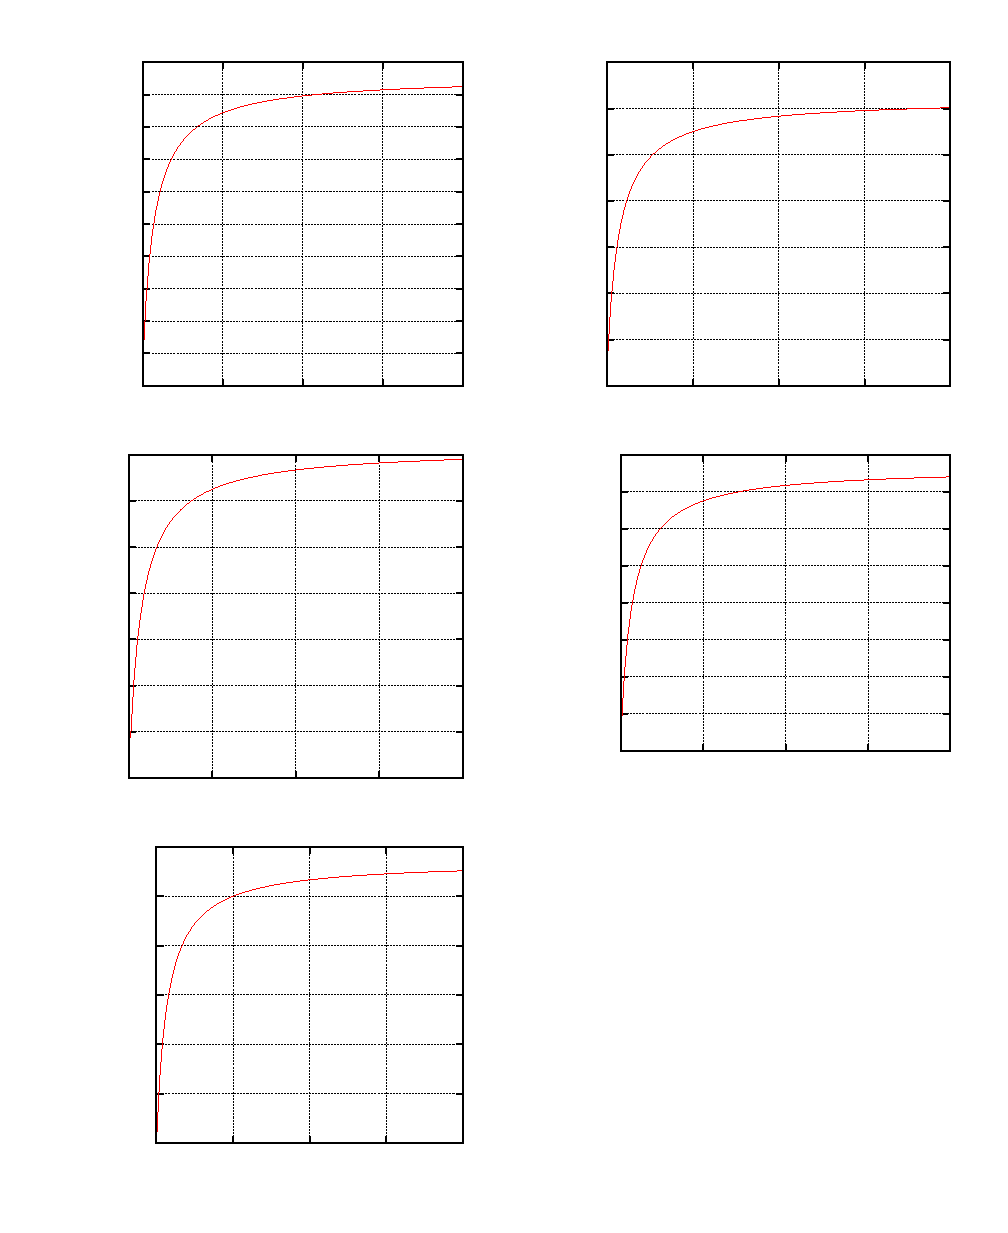
\includegraphics{./figures/oct_edge}}%
    \gplfronttext
  \end{picture}%
\endgroup

\caption{Kante Oktaeder}
\end{figure}
\newpage

\begin{landscape}
\section{Anhang: Gleichungssysteme und zugehörige Schaltpläne}
\subsection{Würfel}

\subsubsection{Spannung an der Raumdiagonalen}
\begin{align}
\begin{pmatrix}
R_1+R_2+R_3+R_4 &  -R_4  &  0  &  -R_3  &  -R_2  &  0  \\ 
-R_4 & R_4+R_6+R_7+R_{10} & -R_{10} & -R_7 & -R_6 & -R_6 \\ 
 0  & -R_{10} & R_9+R_{10}+R_{11}+R_{12} & -R_{11} & -R_9 & -(R_9+R_{12}) \\ 
-R_3 & -R_7 & -R_11 & R_3+R_7+R_8+R_{11} & 0 & 0 \\ 
-R_2 & -R_6 & -R_9 & 0 & R_2+R_5+R_6+R_9 & R_6+R_9 \\ 
 0  & -R_6 & -(R_9+R_{12}) &  0  & R_6+R_9 & R_6+R_9+R_{12}
\end{pmatrix}
\begin{pmatrix}
I_1\\I_2\\I_3\\I_4\\I_5\\I_{ges}
\end{pmatrix}
=
\begin{pmatrix}
0\\0\\0\\0\\0\\U
\end{pmatrix}
\label{eqn:wuerfel_ganz}
\end{align}
\thispagestyle{empty}
\begin{figure}[htbp!]
\centering
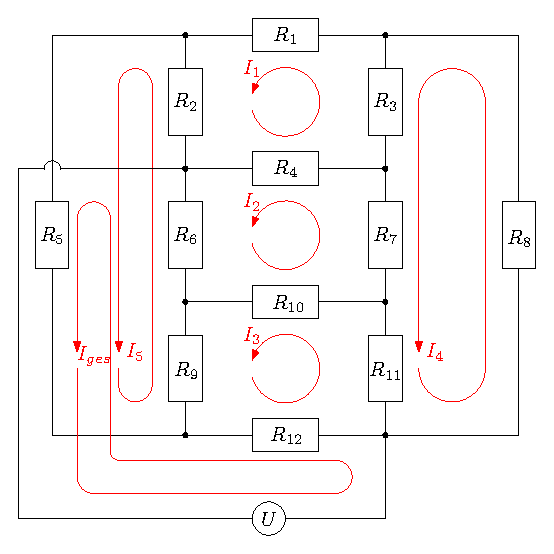
\includegraphics{./figures/wuerfel_schaltplan.eps}
\caption{Schaltplan eines Widerstandswürfels mit angelegter Spannung an einer Raumdiagonalen}
\label{fig:wuerfel_schaltplan}
\end{figure}

\subsubsection{Spannung an der Flächendiagonalen}

\begin{align}
\begin{pmatrix}
R_1+R_2+R_3+R_4 &  -R_4  &  0  &  -R_3  &  -R_2  &  0  \\ 
-R_4 & R_4+R_6+R_7+R_{10} & -R_{10} & -R_7 & -R_6 & -R_6 \\ 
 0  & -R_{10} & R_9+R_{10}+R_{11}+R_{12} & -R_{11} & -R_9 & -R_9 \\ 
-R_3 & -R_7 & -R_11 & R_3+R_7+R_8+R_{11} & 0 & 0 \\ 
-R_2 & -R_6 & -R_9 & 0 & R_2+R_5+R_6+R_9 & R_6+R_9 \\ 
 0  & -R_6 & -R_9 &  0  & R_6+R_9 & R_6+R_9
\end{pmatrix}
\begin{pmatrix}
I_1\\I_2\\I_3\\I_4\\I_5\\I_{ges}
\end{pmatrix}
=
\begin{pmatrix}
0\\0\\0\\0\\0\\U
\end{pmatrix}
\label{eqn:wuerfel_flaeche}
\end{align}
\thispagestyle{empty}

\begin{figure}[htbp!]
\centering
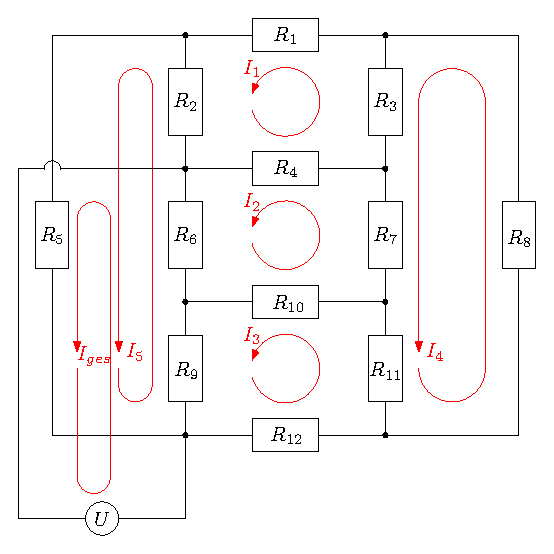
\includegraphics{./figures/wuerfel_schaltplan_flaeche.eps}
\caption{Schaltplan eines Widerstandswürfels mit angelegter Spannung an einer Flächendiagonalen}
\label{fig:wuerfel_schaltplan_flaeche}
\end{figure}

\subsubsection{Spannung an einer Kante}
\begin{align}
\begin{pmatrix}
R_1+R_2+R_3+R_4 &  -R_4  &  0  &  -R_3  &  -R_2  &  0  \\ 
-R_4 & R_4+R_6+R_7+R_{10} & -R_{10} & -R_7 & -R_6 & 0 \\ 
 0  & -R_{10} & R_9+R_{10}+R_{11}+R_{12} & -R_{11} & -R_9 & -R_{12} \\ 
-R_3 & -R_7 & -R_11 & R_3+R_7+R_8+R_{11} & 0 & 0 \\ 
-R_2 & -R_6 & -R_9 & 0 & R_2+R_5+R_6+R_9 & 0 \\ 
 0  & 0 & -R_{12} &  0  & 0 & R_{12}
\end{pmatrix}
\begin{pmatrix}
I_1\\I_2\\I_3\\I_4\\I_5\\I_{ges}
\end{pmatrix}
=
\begin{pmatrix}
0\\0\\0\\0\\0\\U
\end{pmatrix}
\label{eqn:querfel_kante}
\end{align}
\thispagestyle{empty}
\begin{figure}[htbp!]
\centering
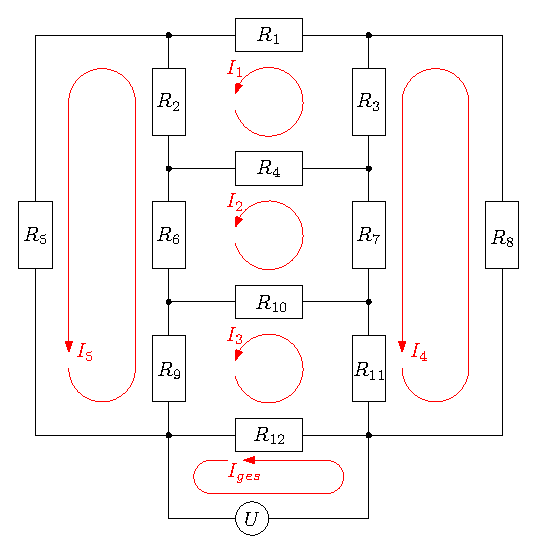
\includegraphics{./figures/wuerfel_schaltplan_kante.eps}
\caption{Schaltplan eines Widerstandswürfels mit angelegter Spannung an einer Kante}
\label{fig:wuerfel_schaltplan_kante}
\end{figure}
\subsection{Oktaeder}

\subsubsection{Spannung an der Diagonalen}
\begin{align}
\begin{pmatrix}
	0 & 0 & -R_4 & 0 & 0 & -R_{12} & 0 & R_4 + R_{12} \\
	R_1 + R_2 + R_5 & -R_2 & 0 & -R_5 & 0 & 0 &-R_5 & 0 \\
	-R_2 & R_2 + R_3 + R_6 & -R_3 & 0 & -R_6 & 0 & -R_6 & 0 \\
	0 & -R_3 & R_3 + R_4 + R_7 & 0 & 0 & -R_7 & -R_7 & -R_4 \\
	-R_5 & 0 & 0 & R_5 + R_9 + R_{10} & -R_{10} & 0 & R_5 & 0 \\
	0 & -R_6 & 0 & -R_{10} & R_6 + R_{10} + R_{11} & -R_{11} & R_6 & 0 \\
	0 & 0 & -R_7 & 0 & -R_{11} & R_7 + R_{11} + R_{12} & R_7 & -R_{12} \\
	-R_5 & -R_6 & -R_7 & R_5 & R_6 & R_7 & R_5 + R_6 + R_7 + R_8 & 0
\end{pmatrix}
\begin{pmatrix}
I_1\\ I_2\\ I_3\\I_4\\I_5\\I_6\\I_7\\I_{ges}
\end{pmatrix}
=
\begin{pmatrix}
U\\0\\0\\0\\0\\0\\0\\0
\end{pmatrix}
\label{eqn:oktaeder_ganz}
\end{align}
\begin{figure}[htbp!]
\centering
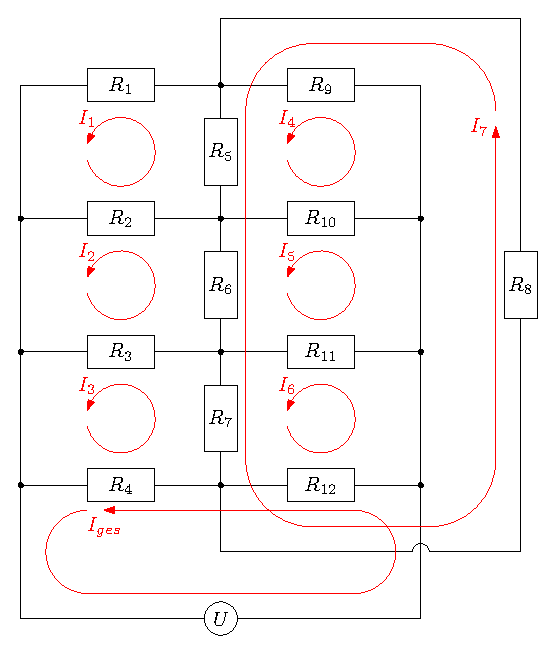
\includegraphics[height=290pt]{./figures/oktaeder_schaltplan.eps}
\caption{Schaltplan eines Oktaeders mit angelegter Spannung an der Raumdiagonalen}
\label{fig:oktaeder_schaltplan}
\end{figure}
\thispagestyle{empty}
\subsubsection{Spannung an einer Kante}

\begin{align}
\begin{pmatrix}
	0 & 0 & -R_4 & 0 & 0 & 0 & 0 & R_4 \\
	R_1 + R_2 + R_5 & -R_2 & 0 & -R_5 & 0 & 0 &-R_5 & 0 \\
	-R_2 & R_2 + R_3 + R_6 & -R_3 & 0 & -R_6 & 0 & -R_6 & 0 \\
	0 & -R_3 & R_3 + R_4 + R_7 & 0 & 0 & -R_7 & -R_7 & -R_4 \\
	-R_5 & 0 & 0 & R_5 + R_9 + R_{10} & -R_{10} & 0 & R_5 & 0 \\
	0 & -R_6 & 0 & -R_{10} & R_6 + R_{10} + R_{11} & -R_{11} & R_6 & 0 \\
	0 & 0 & -R_7 & 0 & -R_{11} & R_7 + R_{11} + R_{12} & R_7 & 0 \\
	-R_5 & -R_6 & -R_7 & R_5 & R_6 & R_7 & R_5 + R_6 + R_7 + R_8 & 0
\end{pmatrix}
\begin{pmatrix}
I_1\\ I_2\\ I_3\\I_4\\I_5\\I_6\\I_7\\I_{ges}
\end{pmatrix}
=
\begin{pmatrix}
U\\0\\0\\0\\0\\0\\0\\0
\end{pmatrix}
\end{align}
\thispagestyle{empty}
\begin{figure}[htbp!]
\centering
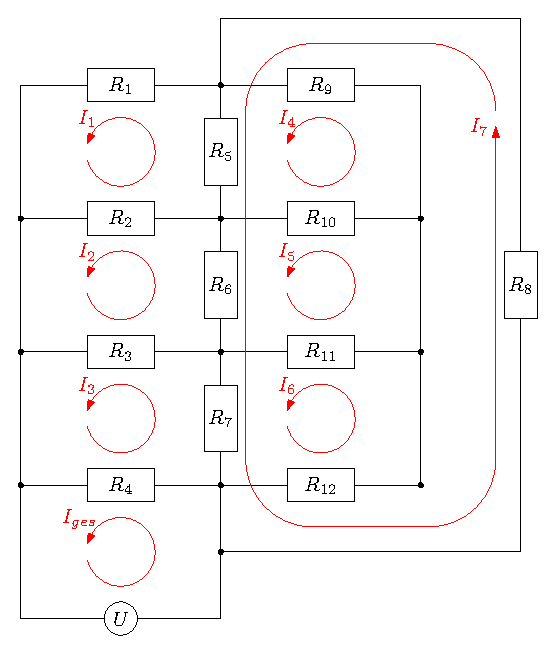
\includegraphics[height=290pt]{./figures/oktaeder_schaltplan_kante.eps}
\caption{Schaltplan eines Oktaeders mit angelegter Spannung an einer Kante}
\label{fig:oktaeder_schaltplan_kante}
\end{figure}
\end{landscape}

\end{document}
